\documentclass[twoside]{book}

% Packages required by doxygen
\usepackage{fixltx2e}
\usepackage{calc}
\usepackage{doxygen}
\usepackage[export]{adjustbox} % also loads graphicx
\usepackage{graphicx}
\usepackage[utf8]{inputenc}
\usepackage{makeidx}
\usepackage{multicol}
\usepackage{multirow}
\PassOptionsToPackage{warn}{textcomp}
\usepackage{textcomp}
\usepackage[nointegrals]{wasysym}
\usepackage[table]{xcolor}

% Font selection
\usepackage[T1]{fontenc}
\usepackage[scaled=.90]{helvet}
\usepackage{courier}
\usepackage{amssymb}
\usepackage{sectsty}
\renewcommand{\familydefault}{\sfdefault}
\allsectionsfont{%
  \fontseries{bc}\selectfont%
  \color{darkgray}%
}
\renewcommand{\DoxyLabelFont}{%
  \fontseries{bc}\selectfont%
  \color{darkgray}%
}
\newcommand{\+}{\discretionary{\mbox{\scriptsize$\hookleftarrow$}}{}{}}

% Page & text layout
\usepackage{geometry}
\geometry{%
  a4paper,%
  top=2.5cm,%
  bottom=2.5cm,%
  left=2.5cm,%
  right=2.5cm%
}
\tolerance=750
\hfuzz=15pt
\hbadness=750
\setlength{\emergencystretch}{15pt}
\setlength{\parindent}{0cm}
\setlength{\parskip}{3ex plus 2ex minus 2ex}
\makeatletter
\renewcommand{\paragraph}{%
  \@startsection{paragraph}{4}{0ex}{-1.0ex}{1.0ex}{%
    \normalfont\normalsize\bfseries\SS@parafont%
  }%
}
\renewcommand{\subparagraph}{%
  \@startsection{subparagraph}{5}{0ex}{-1.0ex}{1.0ex}{%
    \normalfont\normalsize\bfseries\SS@subparafont%
  }%
}
\makeatother

% Headers & footers
\usepackage{fancyhdr}
\pagestyle{fancyplain}
\fancyhead[LE]{\fancyplain{}{\bfseries\thepage}}
\fancyhead[CE]{\fancyplain{}{}}
\fancyhead[RE]{\fancyplain{}{\bfseries\leftmark}}
\fancyhead[LO]{\fancyplain{}{\bfseries\rightmark}}
\fancyhead[CO]{\fancyplain{}{}}
\fancyhead[RO]{\fancyplain{}{\bfseries\thepage}}
\fancyfoot[LE]{\fancyplain{}{}}
\fancyfoot[CE]{\fancyplain{}{}}
\fancyfoot[RE]{\fancyplain{}{\bfseries\scriptsize Generated by Doxygen }}
\fancyfoot[LO]{\fancyplain{}{\bfseries\scriptsize Generated by Doxygen }}
\fancyfoot[CO]{\fancyplain{}{}}
\fancyfoot[RO]{\fancyplain{}{}}
\renewcommand{\footrulewidth}{0.4pt}
\renewcommand{\chaptermark}[1]{%
  \markboth{#1}{}%
}
\renewcommand{\sectionmark}[1]{%
  \markright{\thesection\ #1}%
}

% Indices & bibliography
\usepackage{natbib}
\usepackage[titles]{tocloft}
\setcounter{tocdepth}{3}
\setcounter{secnumdepth}{5}
\makeindex

% Hyperlinks (required, but should be loaded last)
\usepackage{ifpdf}
\ifpdf
  \usepackage[pdftex,pagebackref=true]{hyperref}
\else
  \usepackage[ps2pdf,pagebackref=true]{hyperref}
\fi
\hypersetup{%
  colorlinks=true,%
  linkcolor=blue,%
  citecolor=blue,%
  unicode%
}

% Custom commands
\newcommand{\clearemptydoublepage}{%
  \newpage{\pagestyle{empty}\cleardoublepage}%
}

\usepackage{caption}
\captionsetup{labelsep=space,justification=centering,font={bf},singlelinecheck=off,skip=4pt,position=top}

%===== C O N T E N T S =====

\begin{document}

% Titlepage & ToC
\hypersetup{pageanchor=false,
             bookmarksnumbered=true,
             pdfencoding=unicode
            }
\pagenumbering{roman}
\begin{titlepage}
\vspace*{7cm}
\begin{center}%
{\Large Assignment1.1 \\[1ex]\large 1.\+1 }\\
\vspace*{1cm}
{\large Generated by Doxygen 1.8.11}\\
\end{center}
\end{titlepage}
\clearemptydoublepage
\tableofcontents
\clearemptydoublepage
\pagenumbering{arabic}
\hypersetup{pageanchor=true}

%--- Begin generated contents ---
\chapter{Hierarchical Index}
\section{Class Hierarchy}
This inheritance list is sorted roughly, but not completely, alphabetically\+:\begin{DoxyCompactList}
\item \contentsline{section}{Test.\+Bishop\+Test}{\pageref{class_test_1_1_bishop_test}}{}
\item \contentsline{section}{Board\+And\+Game.\+Board}{\pageref{class_board_and_game_1_1_board}}{}
\item \contentsline{section}{Test.\+Board\+Test}{\pageref{class_test_1_1_board_test}}{}
\item \contentsline{section}{Board\+And\+Game.\+Chess\+Game}{\pageref{class_board_and_game_1_1_chess_game}}{}
\item \contentsline{section}{Chess\+Pieces.\+Chess\+Piece}{\pageref{class_chess_pieces_1_1_chess_piece}}{}
\begin{DoxyCompactList}
\item \contentsline{section}{Chess\+Pieces.\+Bishop}{\pageref{class_chess_pieces_1_1_bishop}}{}
\item \contentsline{section}{Chess\+Pieces.\+King}{\pageref{class_chess_pieces_1_1_king}}{}
\item \contentsline{section}{Chess\+Pieces.\+Knight}{\pageref{class_chess_pieces_1_1_knight}}{}
\item \contentsline{section}{Chess\+Pieces.\+Pawn}{\pageref{class_chess_pieces_1_1_pawn}}{}
\item \contentsline{section}{Chess\+Pieces.\+Queen}{\pageref{class_chess_pieces_1_1_queen}}{}
\item \contentsline{section}{Chess\+Pieces.\+Rook}{\pageref{class_chess_pieces_1_1_rook}}{}
\end{DoxyCompactList}
\item \contentsline{section}{Chess\+Pieces.\+Color}{\pageref{enum_chess_pieces_1_1_color}}{}
\item \contentsline{section}{Test.\+King\+Test}{\pageref{class_test_1_1_king_test}}{}
\item \contentsline{section}{Test.\+Knight\+Test}{\pageref{class_test_1_1_knight_test}}{}
\item \contentsline{section}{Chess\+Pieces.\+Location}{\pageref{class_chess_pieces_1_1_location}}{}
\item \contentsline{section}{Chess\+Pieces.\+Movement}{\pageref{class_chess_pieces_1_1_movement}}{}
\item \contentsline{section}{Test.\+Pawn\+Test}{\pageref{class_test_1_1_pawn_test}}{}
\item \contentsline{section}{Test.\+Queen\+Test}{\pageref{class_test_1_1_queen_test}}{}
\item \contentsline{section}{Test.\+Rook\+Test}{\pageref{class_test_1_1_rook_test}}{}
\item \contentsline{section}{Board\+And\+Game.\+Square}{\pageref{class_board_and_game_1_1_square}}{}
\end{DoxyCompactList}

\chapter{Class Index}
\section{Class List}
Here are the classes, structs, unions and interfaces with brief descriptions\+:\begin{DoxyCompactList}
\item\contentsline{section}{\hyperlink{class_chess_pieces_1_1_bishop}{Chess\+Pieces.\+Bishop} }{\pageref{class_chess_pieces_1_1_bishop}}{}
\item\contentsline{section}{\hyperlink{class_test_1_1_bishop_test}{Test.\+Bishop\+Test} }{\pageref{class_test_1_1_bishop_test}}{}
\item\contentsline{section}{\hyperlink{class_board_and_game_1_1_board}{Board\+And\+Game.\+Board} }{\pageref{class_board_and_game_1_1_board}}{}
\item\contentsline{section}{\hyperlink{class_test_1_1_board_test}{Test.\+Board\+Test} }{\pageref{class_test_1_1_board_test}}{}
\item\contentsline{section}{\hyperlink{class_board_and_game_1_1_chess_game}{Board\+And\+Game.\+Chess\+Game} }{\pageref{class_board_and_game_1_1_chess_game}}{}
\item\contentsline{section}{\hyperlink{class_chess_pieces_1_1_chess_piece}{Chess\+Pieces.\+Chess\+Piece} }{\pageref{class_chess_pieces_1_1_chess_piece}}{}
\item\contentsline{section}{\hyperlink{enum_chess_pieces_1_1_color}{Chess\+Pieces.\+Color} }{\pageref{enum_chess_pieces_1_1_color}}{}
\item\contentsline{section}{\hyperlink{class_chess_pieces_1_1_king}{Chess\+Pieces.\+King} }{\pageref{class_chess_pieces_1_1_king}}{}
\item\contentsline{section}{\hyperlink{class_test_1_1_king_test}{Test.\+King\+Test} }{\pageref{class_test_1_1_king_test}}{}
\item\contentsline{section}{\hyperlink{class_chess_pieces_1_1_knight}{Chess\+Pieces.\+Knight} }{\pageref{class_chess_pieces_1_1_knight}}{}
\item\contentsline{section}{\hyperlink{class_test_1_1_knight_test}{Test.\+Knight\+Test} }{\pageref{class_test_1_1_knight_test}}{}
\item\contentsline{section}{\hyperlink{class_chess_pieces_1_1_location}{Chess\+Pieces.\+Location} }{\pageref{class_chess_pieces_1_1_location}}{}
\item\contentsline{section}{\hyperlink{class_chess_pieces_1_1_movement}{Chess\+Pieces.\+Movement} }{\pageref{class_chess_pieces_1_1_movement}}{}
\item\contentsline{section}{\hyperlink{class_chess_pieces_1_1_pawn}{Chess\+Pieces.\+Pawn} }{\pageref{class_chess_pieces_1_1_pawn}}{}
\item\contentsline{section}{\hyperlink{class_test_1_1_pawn_test}{Test.\+Pawn\+Test} }{\pageref{class_test_1_1_pawn_test}}{}
\item\contentsline{section}{\hyperlink{class_chess_pieces_1_1_queen}{Chess\+Pieces.\+Queen} }{\pageref{class_chess_pieces_1_1_queen}}{}
\item\contentsline{section}{\hyperlink{class_test_1_1_queen_test}{Test.\+Queen\+Test} }{\pageref{class_test_1_1_queen_test}}{}
\item\contentsline{section}{\hyperlink{class_chess_pieces_1_1_rook}{Chess\+Pieces.\+Rook} }{\pageref{class_chess_pieces_1_1_rook}}{}
\item\contentsline{section}{\hyperlink{class_test_1_1_rook_test}{Test.\+Rook\+Test} }{\pageref{class_test_1_1_rook_test}}{}
\item\contentsline{section}{\hyperlink{class_board_and_game_1_1_square}{Board\+And\+Game.\+Square} }{\pageref{class_board_and_game_1_1_square}}{}
\end{DoxyCompactList}

\chapter{Class Documentation}
\hypertarget{class_chess_pieces_1_1_bishop}{}\section{Chess\+Pieces.\+Bishop Class Reference}
\label{class_chess_pieces_1_1_bishop}\index{Chess\+Pieces.\+Bishop@{Chess\+Pieces.\+Bishop}}
Inheritance diagram for Chess\+Pieces.\+Bishop\+:\begin{figure}[H]
\begin{center}
\leavevmode
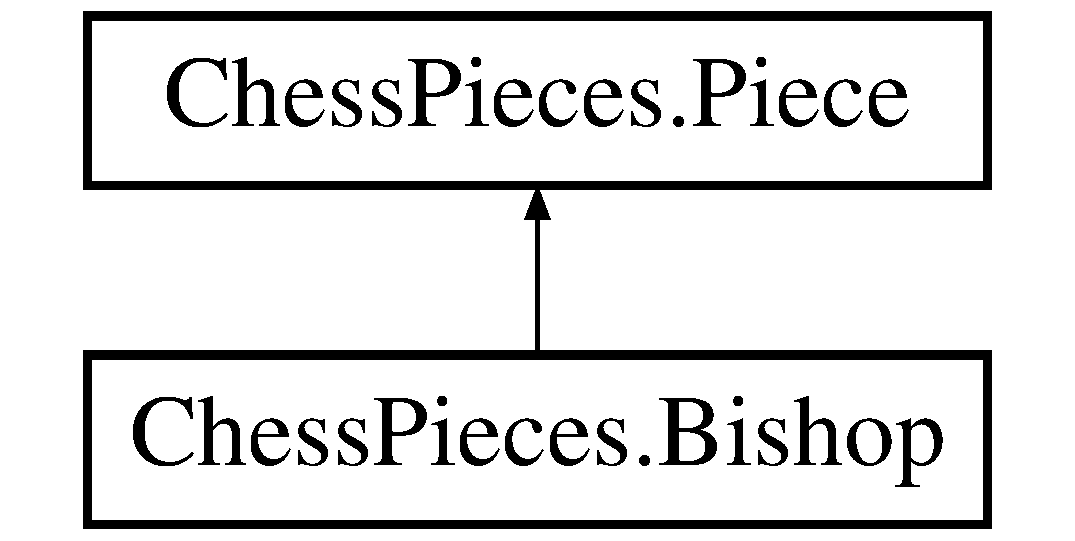
\includegraphics[height=2.000000cm]{class_chess_pieces_1_1_bishop}
\end{center}
\end{figure}
\subsection*{Public Member Functions}
\begin{DoxyCompactItemize}
\item 
{\bfseries Bishop} (\hyperlink{enum_chess_pieces_1_1_color}{Color} col, \hyperlink{class_chess_pieces_1_1_location}{Location} loc)\hypertarget{class_chess_pieces_1_1_bishop_a29778e28497c7cbba679f1f12864f54b}{}\label{class_chess_pieces_1_1_bishop_a29778e28497c7cbba679f1f12864f54b}

\item 
boolean {\bfseries can\+Move\+To} (\hyperlink{class_chess_pieces_1_1_location}{Location} dest)\hypertarget{class_chess_pieces_1_1_bishop_a89fbf2408312d3976c8f203fefd49ecd}{}\label{class_chess_pieces_1_1_bishop_a89fbf2408312d3976c8f203fefd49ecd}

\end{DoxyCompactItemize}
\subsection*{Additional Inherited Members}


\subsection{Detailed Description}
Created by admin on 1/29/16. this is the class of \hyperlink{class_chess_pieces_1_1_bishop}{Bishop} 

The documentation for this class was generated from the following file\+:\begin{DoxyCompactItemize}
\item 
src/\+Chess\+Pieces/Bishop.\+java\end{DoxyCompactItemize}

\hypertarget{class_test_1_1_bishop_test}{}\section{Test.\+Bishop\+Test Class Reference}
\label{class_test_1_1_bishop_test}\index{Test.\+Bishop\+Test@{Test.\+Bishop\+Test}}
\subsection*{Public Member Functions}
\begin{DoxyCompactItemize}
\item 
void {\bfseries test\+Can\+Move\+To} ()  throws Exception \hypertarget{class_test_1_1_bishop_test_a2b655d0ca48789dca494415fc652abf2}{}\label{class_test_1_1_bishop_test_a2b655d0ca48789dca494415fc652abf2}

\end{DoxyCompactItemize}


\subsection{Detailed Description}
Created by admin on 2/2/16. 

The documentation for this class was generated from the following file\+:\begin{DoxyCompactItemize}
\item 
src/\+Test/Bishop\+Test.\+java\end{DoxyCompactItemize}

\hypertarget{class_board_and_game_1_1_board}{}\section{Board\+And\+Game.\+Board Class Reference}
\label{class_board_and_game_1_1_board}\index{Board\+And\+Game.\+Board@{Board\+And\+Game.\+Board}}
\subsection*{Public Member Functions}
\begin{DoxyCompactItemize}
\item 
{\bfseries Board} (int x, int y)\hypertarget{class_board_and_game_1_1_board_a1428f0b186268c8ad2ac05565037ff31}{}\label{class_board_and_game_1_1_board_a1428f0b186268c8ad2ac05565037ff31}

\item 
boolean {\bfseries no\+Piece\+In\+The\+Middle} (\hyperlink{class_chess_pieces_1_1_location}{Location} start, \hyperlink{class_chess_pieces_1_1_location}{Location} dest)\hypertarget{class_board_and_game_1_1_board_ae89018c37930d36db7dcb78e0bcea6d5}{}\label{class_board_and_game_1_1_board_ae89018c37930d36db7dcb78e0bcea6d5}

\item 
boolean {\bfseries is\+Inside\+Board} (\hyperlink{class_chess_pieces_1_1_location}{Location} dest)\hypertarget{class_board_and_game_1_1_board_aec226eaa8db092c90b4f2dbfa647565d}{}\label{class_board_and_game_1_1_board_aec226eaa8db092c90b4f2dbfa647565d}

\item 
boolean {\bfseries capture\+Opponent} (\hyperlink{class_chess_pieces_1_1_location}{Location} start, \hyperlink{class_chess_pieces_1_1_location}{Location} dest)\hypertarget{class_board_and_game_1_1_board_ae7074c4740ef7c9f850c5aa3e8cbdacd}{}\label{class_board_and_game_1_1_board_ae7074c4740ef7c9f850c5aa3e8cbdacd}

\item 
boolean {\bfseries go\+To} (\hyperlink{class_chess_pieces_1_1_location}{Location} start, \hyperlink{class_chess_pieces_1_1_location}{Location} dest)\hypertarget{class_board_and_game_1_1_board_a2175dfc362422b753bd0f8ec55dd50f4}{}\label{class_board_and_game_1_1_board_a2175dfc362422b753bd0f8ec55dd50f4}

\item 
boolean {\bfseries check\+Mate} (\hyperlink{enum_chess_pieces_1_1_color}{Color} Opponent\+Color)\hypertarget{class_board_and_game_1_1_board_ad922490ab63ddb125c7eda9487957720}{}\label{class_board_and_game_1_1_board_ad922490ab63ddb125c7eda9487957720}

\item 
boolean {\bfseries Check\+Blocks\+And\+Kills} (\hyperlink{class_chess_pieces_1_1_chess_piece}{Chess\+Piece} opponent\+King, Array\+List$<$ \hyperlink{class_chess_pieces_1_1_chess_piece}{Chess\+Piece} $>$ my\+Pieces, Array\+List$<$ \hyperlink{class_chess_pieces_1_1_chess_piece}{Chess\+Piece} $>$ opponent\+Pieces)\hypertarget{class_board_and_game_1_1_board_a6e45ab270b5ee8cecd191a3cf380b1e5}{}\label{class_board_and_game_1_1_board_a6e45ab270b5ee8cecd191a3cf380b1e5}

\item 
boolean {\bfseries in\+Check} (\hyperlink{class_chess_pieces_1_1_chess_piece}{Chess\+Piece} opponent\+King, Array\+List$<$ \hyperlink{class_chess_pieces_1_1_chess_piece}{Chess\+Piece} $>$ my\+Pieces, Array\+List$<$ \hyperlink{class_chess_pieces_1_1_chess_piece}{Chess\+Piece} $>$ opponent\+Pieces)\hypertarget{class_board_and_game_1_1_board_a8446160245d5c189c3875a9511f727ec}{}\label{class_board_and_game_1_1_board_a8446160245d5c189c3875a9511f727ec}

\item 
boolean \hyperlink{class_board_and_game_1_1_board_aca2ba816fbc7e6281ae9fa5f07f99fe9}{can\+Move\+To} (\hyperlink{class_chess_pieces_1_1_location}{Location} start, \hyperlink{class_chess_pieces_1_1_location}{Location} dest)
\item 
boolean {\bfseries can\+Move\+To\+With\+Block} (\hyperlink{class_chess_pieces_1_1_location}{Location} start, \hyperlink{class_chess_pieces_1_1_location}{Location} dest, Array\+List$<$ \hyperlink{class_chess_pieces_1_1_chess_piece}{Chess\+Piece} $>$ opponent\+Chess)\hypertarget{class_board_and_game_1_1_board_af69f26e31d18896274d8ef21a39488b8}{}\label{class_board_and_game_1_1_board_af69f26e31d18896274d8ef21a39488b8}

\item 
\hyperlink{class_chess_pieces_1_1_chess_piece}{Chess\+Piece} {\bfseries get\+Chess\+Piece} (\hyperlink{class_chess_pieces_1_1_location}{Location} location)\hypertarget{class_board_and_game_1_1_board_a9923a7cad02defefd058588120bd45e6}{}\label{class_board_and_game_1_1_board_a9923a7cad02defefd058588120bd45e6}

\item 
\hyperlink{class_board_and_game_1_1_square}{Square} {\bfseries get\+Square} (\hyperlink{class_chess_pieces_1_1_location}{Location} location)\hypertarget{class_board_and_game_1_1_board_a71e3336b3e67e2aa0833cbb1863651bd}{}\label{class_board_and_game_1_1_board_a71e3336b3e67e2aa0833cbb1863651bd}

\item 
Array\+List$<$ \hyperlink{class_chess_pieces_1_1_location}{Location} $>$ {\bfseries get\+Location\+Around\+It} (\hyperlink{class_chess_pieces_1_1_location}{Location} location)\hypertarget{class_board_and_game_1_1_board_affb2904486fde6fff180ac997e01f1cd}{}\label{class_board_and_game_1_1_board_affb2904486fde6fff180ac997e01f1cd}

\item 
Array\+List$<$ \hyperlink{class_chess_pieces_1_1_location}{Location} $>$ {\bfseries get\+Location\+In\+The\+Middle} (\hyperlink{class_chess_pieces_1_1_location}{Location} start, \hyperlink{class_chess_pieces_1_1_location}{Location} dest)\hypertarget{class_board_and_game_1_1_board_a85ec1c66d5c24efc1b829ea56fb91ccd}{}\label{class_board_and_game_1_1_board_a85ec1c66d5c24efc1b829ea56fb91ccd}

\item 
void {\bfseries test\+Go\+To} (\hyperlink{class_chess_pieces_1_1_location}{Location} start, \hyperlink{class_chess_pieces_1_1_location}{Location} dest)\hypertarget{class_board_and_game_1_1_board_a381092c0a3eb63365acaad6098ad3adc}{}\label{class_board_and_game_1_1_board_a381092c0a3eb63365acaad6098ad3adc}

\item 
void {\bfseries test\+Delete} (\hyperlink{class_chess_pieces_1_1_location}{Location} a)\hypertarget{class_board_and_game_1_1_board_a73bea789be1ef022a3bdde4dfec45abc}{}\label{class_board_and_game_1_1_board_a73bea789be1ef022a3bdde4dfec45abc}

\item 
Array\+List$<$ \hyperlink{class_chess_pieces_1_1_chess_piece}{Chess\+Piece} $>$ {\bfseries test\+Get\+White\+Pieces} ()\hypertarget{class_board_and_game_1_1_board_a9a9d62c6cb54db0900fb4fdbf9631730}{}\label{class_board_and_game_1_1_board_a9a9d62c6cb54db0900fb4fdbf9631730}

\item 
Array\+List$<$ \hyperlink{class_chess_pieces_1_1_chess_piece}{Chess\+Piece} $>$ {\bfseries test\+Get\+Black\+Pieces} ()\hypertarget{class_board_and_game_1_1_board_ace2944e1ea40b215d62ffc8572ef9c0b}{}\label{class_board_and_game_1_1_board_ace2944e1ea40b215d62ffc8572ef9c0b}

\end{DoxyCompactItemize}
\subsection*{Protected Attributes}
\begin{DoxyCompactItemize}
\item 
\hyperlink{class_board_and_game_1_1_square}{Square}\mbox{[}$\,$\mbox{]}\mbox{[}$\,$\mbox{]} {\bfseries squares}\hypertarget{class_board_and_game_1_1_board_adf1bbfe988dc243bb6989ae574ee8c2c}{}\label{class_board_and_game_1_1_board_adf1bbfe988dc243bb6989ae574ee8c2c}

\item 
int {\bfseries column}\hypertarget{class_board_and_game_1_1_board_adb554a7959da1c68ee659ad4b9a87bef}{}\label{class_board_and_game_1_1_board_adb554a7959da1c68ee659ad4b9a87bef}

\item 
int {\bfseries row}\hypertarget{class_board_and_game_1_1_board_a1a812ca2e5aba395e1da106f8a3506d7}{}\label{class_board_and_game_1_1_board_a1a812ca2e5aba395e1da106f8a3506d7}

\item 
Array\+List$<$ \hyperlink{class_chess_pieces_1_1_chess_piece}{Chess\+Piece} $>$ {\bfseries white\+Pieces}\hypertarget{class_board_and_game_1_1_board_a8fc6425a96cb7bfb711557557e606db1}{}\label{class_board_and_game_1_1_board_a8fc6425a96cb7bfb711557557e606db1}

\item 
Array\+List$<$ \hyperlink{class_chess_pieces_1_1_chess_piece}{Chess\+Piece} $>$ {\bfseries black\+Pieces}\hypertarget{class_board_and_game_1_1_board_a227b297e707f685da921b58ecf60d509}{}\label{class_board_and_game_1_1_board_a227b297e707f685da921b58ecf60d509}

\end{DoxyCompactItemize}


\subsection{Detailed Description}
Created by Blaks on 1/29/16. 

\subsection{Member Function Documentation}
\index{Board\+And\+Game\+::\+Board@{Board\+And\+Game\+::\+Board}!can\+Move\+To@{can\+Move\+To}}
\index{can\+Move\+To@{can\+Move\+To}!Board\+And\+Game\+::\+Board@{Board\+And\+Game\+::\+Board}}
\subsubsection[{\texorpdfstring{can\+Move\+To(\+Location start, Location dest)}{canMoveTo(Location start, Location dest)}}]{\setlength{\rightskip}{0pt plus 5cm}boolean Board\+And\+Game.\+Board.\+can\+Move\+To (
\begin{DoxyParamCaption}
\item[{{\bf Location}}]{start, }
\item[{{\bf Location}}]{dest}
\end{DoxyParamCaption}
)}\hypertarget{class_board_and_game_1_1_board_aca2ba816fbc7e6281ae9fa5f07f99fe9}{}\label{class_board_and_game_1_1_board_aca2ba816fbc7e6281ae9fa5f07f99fe9}
this function checks whether a piece on a place can move to another place 
\begin{DoxyParams}{Parameters}
{\em start} & \\
\hline
{\em dest} & \\
\hline
\end{DoxyParams}
\begin{DoxyReturn}{Returns}

\end{DoxyReturn}


The documentation for this class was generated from the following file\+:\begin{DoxyCompactItemize}
\item 
src/\+Board\+And\+Game/Board.\+java\end{DoxyCompactItemize}

\hypertarget{class_test_1_1_board_test}{}\section{Test.\+Board\+Test Class Reference}
\label{class_test_1_1_board_test}\index{Test.\+Board\+Test@{Test.\+Board\+Test}}
\subsection*{Public Member Functions}
\begin{DoxyCompactItemize}
\item 
void {\bfseries testgo\+To} ()  throws Exception \hypertarget{class_test_1_1_board_test_ad3cf19d6b94ee85902f7704c05e5294d}{}\label{class_test_1_1_board_test_ad3cf19d6b94ee85902f7704c05e5294d}

\item 
void {\bfseries test\+No\+Piece\+In\+The\+Middle\+Straight} ()  throws Exception \hypertarget{class_test_1_1_board_test_a3eab64f0df28ffebed0c61349263df9d}{}\label{class_test_1_1_board_test_a3eab64f0df28ffebed0c61349263df9d}

\item 
void {\bfseries test\+Is\+Inside\+Board} ()  throws Exception \hypertarget{class_test_1_1_board_test_a6abda7d92957be54facfd5fdc19d6892}{}\label{class_test_1_1_board_test_a6abda7d92957be54facfd5fdc19d6892}

\item 
void {\bfseries test\+Check\+Mate\+Single\+King} ()  throws Exception \hypertarget{class_test_1_1_board_test_a6064fb15fe8ebd54fdd3dc1ac7f68f36}{}\label{class_test_1_1_board_test_a6064fb15fe8ebd54fdd3dc1ac7f68f36}

\item 
void {\bfseries test\+Check\+Mate\+With\+Opponent} ()  throws Exception \hypertarget{class_test_1_1_board_test_a7c25087b76fd393e2e4c59c9916b5f78}{}\label{class_test_1_1_board_test_a7c25087b76fd393e2e4c59c9916b5f78}

\item 
void {\bfseries test\+Capture\+Opponent} ()  throws Exception \hypertarget{class_test_1_1_board_test_af72b8885d1779d91c5934a5d107e2e8d}{}\label{class_test_1_1_board_test_af72b8885d1779d91c5934a5d107e2e8d}

\item 
void {\bfseries test\+Check\+Mate} ()  throws Exception \hypertarget{class_test_1_1_board_test_a215603d80780d0b07b1ad7efdc290503}{}\label{class_test_1_1_board_test_a215603d80780d0b07b1ad7efdc290503}

\item 
void {\bfseries test\+Can\+Move\+To} ()  throws Exception \hypertarget{class_test_1_1_board_test_a1884f81736b1ece2c9b054205ce5b91b}{}\label{class_test_1_1_board_test_a1884f81736b1ece2c9b054205ce5b91b}

\item 
void {\bfseries test\+Can\+Move\+To\+With\+Block} ()  throws Exception \hypertarget{class_test_1_1_board_test_a8b018a6245b67905b815757c0a44d95a}{}\label{class_test_1_1_board_test_a8b018a6245b67905b815757c0a44d95a}

\end{DoxyCompactItemize}


\subsection{Detailed Description}
Created by admin on 2/3/16. 

The documentation for this class was generated from the following file\+:\begin{DoxyCompactItemize}
\item 
src/\+Test/Board\+Test.\+java\end{DoxyCompactItemize}

\hypertarget{class_board_and_game_1_1_chess_game}{}\section{Board\+And\+Game.\+Chess\+Game Class Reference}
\label{class_board_and_game_1_1_chess_game}\index{Board\+And\+Game.\+Chess\+Game@{Board\+And\+Game.\+Chess\+Game}}
\subsection*{Static Public Member Functions}
\begin{DoxyCompactItemize}
\item 
static void {\bfseries main} (String args\mbox{[}$\,$\mbox{]})\hypertarget{class_board_and_game_1_1_chess_game_a8e2766d420f9def40af93816748397d8}{}\label{class_board_and_game_1_1_chess_game_a8e2766d420f9def40af93816748397d8}

\end{DoxyCompactItemize}


\subsection{Detailed Description}
Created by admin on 1/29/16. 

The documentation for this class was generated from the following file\+:\begin{DoxyCompactItemize}
\item 
src/\+Board\+And\+Game/Chess\+Game.\+java\end{DoxyCompactItemize}

\hypertarget{class_chess_pieces_1_1_chess_piece}{}\section{Chess\+Pieces.\+Chess\+Piece Class Reference}
\label{class_chess_pieces_1_1_chess_piece}\index{Chess\+Pieces.\+Chess\+Piece@{Chess\+Pieces.\+Chess\+Piece}}
Inheritance diagram for Chess\+Pieces.\+Chess\+Piece\+:\begin{figure}[H]
\begin{center}
\leavevmode
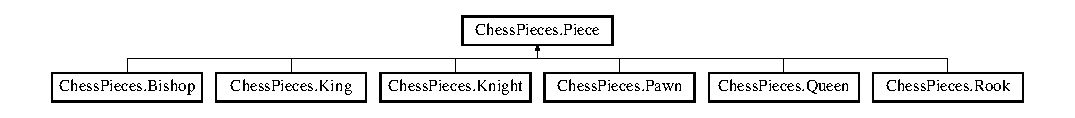
\includegraphics[height=1.138211cm]{class_chess_pieces_1_1_chess_piece}
\end{center}
\end{figure}
\subsection*{Public Member Functions}
\begin{DoxyCompactItemize}
\item 
{\bfseries Chess\+Piece} (\hyperlink{enum_chess_pieces_1_1_color}{Color} col, \hyperlink{class_chess_pieces_1_1_location}{Location} location)\hypertarget{class_chess_pieces_1_1_chess_piece_a10acb1cf463491453995917870d225c8}{}\label{class_chess_pieces_1_1_chess_piece_a10acb1cf463491453995917870d225c8}

\item 
\hyperlink{enum_chess_pieces_1_1_color}{Color} {\bfseries get\+Color} ()\hypertarget{class_chess_pieces_1_1_chess_piece_a8cb8355750b3807abdad1f33bc43bdf4}{}\label{class_chess_pieces_1_1_chess_piece_a8cb8355750b3807abdad1f33bc43bdf4}

\item 
abstract boolean {\bfseries can\+Move\+To} (\hyperlink{class_chess_pieces_1_1_location}{Location} a)\hypertarget{class_chess_pieces_1_1_chess_piece_ab7ef53d95a6778e8e38bfb07861e4c8f}{}\label{class_chess_pieces_1_1_chess_piece_ab7ef53d95a6778e8e38bfb07861e4c8f}

\item 
\hyperlink{class_chess_pieces_1_1_location}{Location} {\bfseries get\+Current\+Location} ()\hypertarget{class_chess_pieces_1_1_chess_piece_ad4528e4dbde0a85ebc8c46b22871aa5c}{}\label{class_chess_pieces_1_1_chess_piece_ad4528e4dbde0a85ebc8c46b22871aa5c}

\item 
void {\bfseries set\+Current\+Location} (\hyperlink{class_chess_pieces_1_1_location}{Location} location)\hypertarget{class_chess_pieces_1_1_chess_piece_aedb67f5f2980ff23efb75ddbd651464d}{}\label{class_chess_pieces_1_1_chess_piece_aedb67f5f2980ff23efb75ddbd651464d}

\end{DoxyCompactItemize}
\subsection*{Protected Attributes}
\begin{DoxyCompactItemize}
\item 
\hyperlink{enum_chess_pieces_1_1_color}{Color} {\bfseries color}\hypertarget{class_chess_pieces_1_1_chess_piece_a06daeee01ede96cd6aa78db766108862}{}\label{class_chess_pieces_1_1_chess_piece_a06daeee01ede96cd6aa78db766108862}

\item 
\hyperlink{class_chess_pieces_1_1_location}{Location} {\bfseries current\+Location}\hypertarget{class_chess_pieces_1_1_chess_piece_a3855d471b3379cc52f7c76898b7cd1da}{}\label{class_chess_pieces_1_1_chess_piece_a3855d471b3379cc52f7c76898b7cd1da}

\end{DoxyCompactItemize}


\subsection{Detailed Description}
Created by Blaks on 1/29/16. 

The documentation for this class was generated from the following file\+:\begin{DoxyCompactItemize}
\item 
src/\+Chess\+Pieces/Chess\+Piece.\+java\end{DoxyCompactItemize}

\hypertarget{enum_chess_pieces_1_1_color}{}\section{Chess\+Pieces.\+Color Enum Reference}
\label{enum_chess_pieces_1_1_color}\index{Chess\+Pieces.\+Color@{Chess\+Pieces.\+Color}}
\subsection*{Public Member Functions}
\begin{DoxyCompactItemize}
\item 
boolean {\bfseries is\+Different} (\hyperlink{enum_chess_pieces_1_1_color}{Color} a, \hyperlink{enum_chess_pieces_1_1_color}{Color} b)\hypertarget{enum_chess_pieces_1_1_color_a5df89f65494839ad057f7d816be87994}{}\label{enum_chess_pieces_1_1_color_a5df89f65494839ad057f7d816be87994}

\item 
boolean {\bfseries is\+White} (\hyperlink{enum_chess_pieces_1_1_color}{Color} a)\hypertarget{enum_chess_pieces_1_1_color_a2eb519654f92a8475317f86edc5a308b}{}\label{enum_chess_pieces_1_1_color_a2eb519654f92a8475317f86edc5a308b}

\item 
boolean {\bfseries is\+Black} (\hyperlink{enum_chess_pieces_1_1_color}{Color} a)\hypertarget{enum_chess_pieces_1_1_color_a9b804db4d208fe8544df533effb3ac36}{}\label{enum_chess_pieces_1_1_color_a9b804db4d208fe8544df533effb3ac36}

\end{DoxyCompactItemize}
\subsection*{Public Attributes}
\begin{DoxyCompactItemize}
\item 
{\bfseries B\+L\+A\+CK}\hypertarget{enum_chess_pieces_1_1_color_a5ad1081ba56bc8cb5a3e0058983ca857}{}\label{enum_chess_pieces_1_1_color_a5ad1081ba56bc8cb5a3e0058983ca857}

\end{DoxyCompactItemize}


\subsection{Detailed Description}
Created by admin on 1/29/16. 

The documentation for this enum was generated from the following file\+:\begin{DoxyCompactItemize}
\item 
src/\+Chess\+Pieces/Color.\+java\end{DoxyCompactItemize}

\hypertarget{class_chess_pieces_1_1_king}{}\section{Chess\+Pieces.\+King Class Reference}
\label{class_chess_pieces_1_1_king}\index{Chess\+Pieces.\+King@{Chess\+Pieces.\+King}}
Inheritance diagram for Chess\+Pieces.\+King\+:\begin{figure}[H]
\begin{center}
\leavevmode
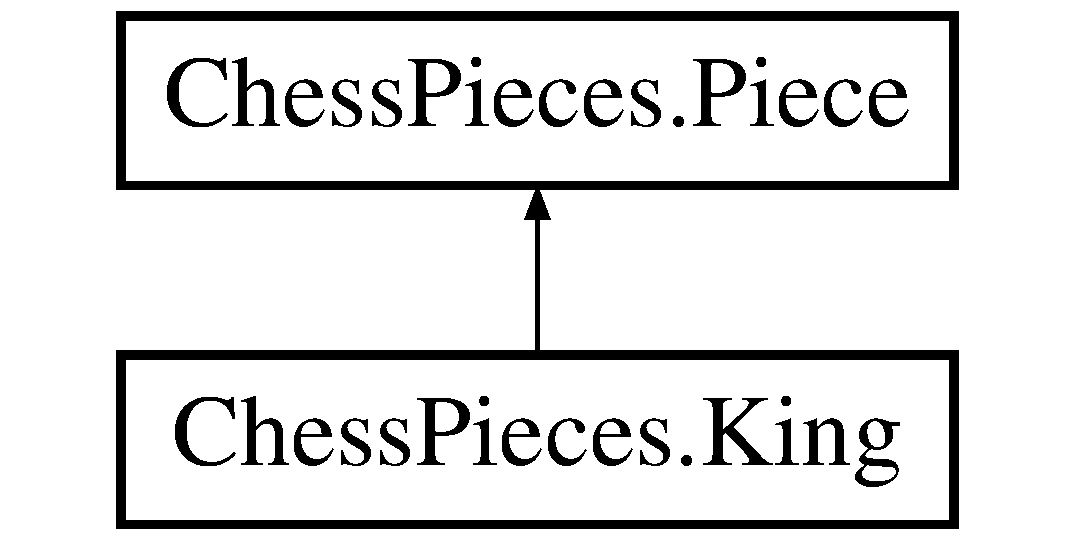
\includegraphics[height=2.000000cm]{class_chess_pieces_1_1_king}
\end{center}
\end{figure}
\subsection*{Public Member Functions}
\begin{DoxyCompactItemize}
\item 
{\bfseries King} (\hyperlink{enum_chess_pieces_1_1_color}{Color} col, \hyperlink{class_chess_pieces_1_1_location}{Location} loc)\hypertarget{class_chess_pieces_1_1_king_a6853b5c75799d9f4662950a9200555fd}{}\label{class_chess_pieces_1_1_king_a6853b5c75799d9f4662950a9200555fd}

\item 
boolean {\bfseries can\+Move\+To} (\hyperlink{class_chess_pieces_1_1_location}{Location} dest)\hypertarget{class_chess_pieces_1_1_king_ae56ded315887600afdf86c03cfae3ae9}{}\label{class_chess_pieces_1_1_king_ae56ded315887600afdf86c03cfae3ae9}

\item 
boolean {\bfseries can\+Castling} ()\hypertarget{class_chess_pieces_1_1_king_a61aa63d17ac310eec5d49c99d30f352d}{}\label{class_chess_pieces_1_1_king_a61aa63d17ac310eec5d49c99d30f352d}

\end{DoxyCompactItemize}
\subsection*{Additional Inherited Members}


\subsection{Detailed Description}
Created by admin on 1/29/16. 

The documentation for this class was generated from the following file\+:\begin{DoxyCompactItemize}
\item 
src/\+Chess\+Pieces/King.\+java\end{DoxyCompactItemize}

\hypertarget{class_test_1_1_king_test}{}\section{Test.\+King\+Test Class Reference}
\label{class_test_1_1_king_test}\index{Test.\+King\+Test@{Test.\+King\+Test}}
\subsection*{Public Member Functions}
\begin{DoxyCompactItemize}
\item 
void {\bfseries test\+Can\+Move\+To} ()  throws Exception \hypertarget{class_test_1_1_king_test_ada4e9cae00e238e4b5a67d7b7402f5a3}{}\label{class_test_1_1_king_test_ada4e9cae00e238e4b5a67d7b7402f5a3}

\end{DoxyCompactItemize}


\subsection{Detailed Description}
Created by admin on 2/2/16. 

The documentation for this class was generated from the following file\+:\begin{DoxyCompactItemize}
\item 
src/\+Test/King\+Test.\+java\end{DoxyCompactItemize}

\hypertarget{class_chess_pieces_1_1_knight}{}\section{Chess\+Pieces.\+Knight Class Reference}
\label{class_chess_pieces_1_1_knight}\index{Chess\+Pieces.\+Knight@{Chess\+Pieces.\+Knight}}
Inheritance diagram for Chess\+Pieces.\+Knight\+:\begin{figure}[H]
\begin{center}
\leavevmode
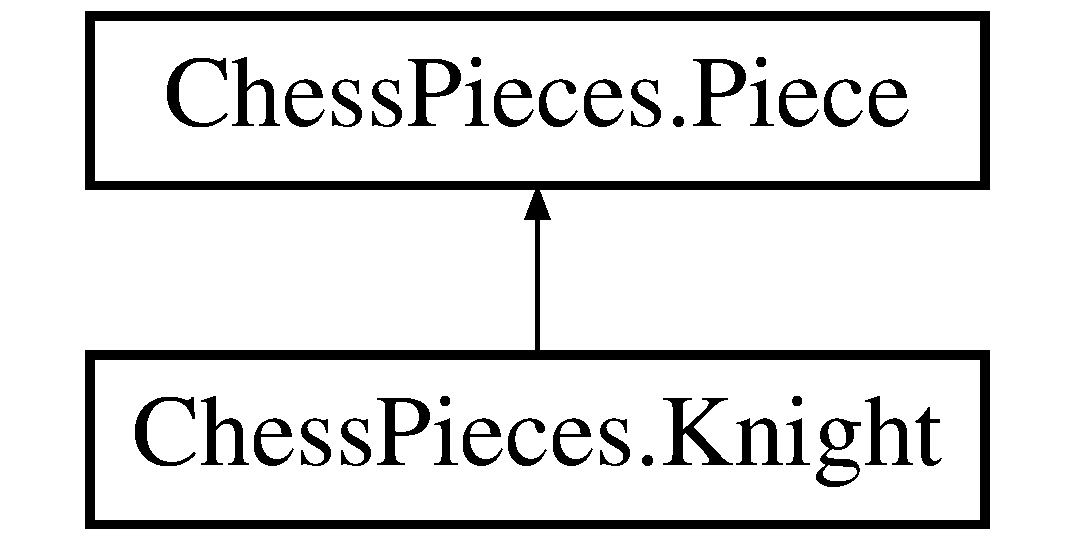
\includegraphics[height=2.000000cm]{class_chess_pieces_1_1_knight}
\end{center}
\end{figure}
\subsection*{Public Member Functions}
\begin{DoxyCompactItemize}
\item 
{\bfseries Knight} (\hyperlink{enum_chess_pieces_1_1_color}{Color} col, \hyperlink{class_chess_pieces_1_1_location}{Location} loc)\hypertarget{class_chess_pieces_1_1_knight_a92ce5e4ffdccb4067075c814b95bf223}{}\label{class_chess_pieces_1_1_knight_a92ce5e4ffdccb4067075c814b95bf223}

\item 
boolean {\bfseries can\+Move\+To} (\hyperlink{class_chess_pieces_1_1_location}{Location} dest)\hypertarget{class_chess_pieces_1_1_knight_a74070aa6822b52e0139e7a92ca6566fc}{}\label{class_chess_pieces_1_1_knight_a74070aa6822b52e0139e7a92ca6566fc}

\end{DoxyCompactItemize}
\subsection*{Additional Inherited Members}


\subsection{Detailed Description}
Created by admin on 1/29/16. 

The documentation for this class was generated from the following file\+:\begin{DoxyCompactItemize}
\item 
src/\+Chess\+Pieces/Knight.\+java\end{DoxyCompactItemize}

\hypertarget{class_test_1_1_knight_test}{}\section{Test.\+Knight\+Test Class Reference}
\label{class_test_1_1_knight_test}\index{Test.\+Knight\+Test@{Test.\+Knight\+Test}}
\subsection*{Public Member Functions}
\begin{DoxyCompactItemize}
\item 
void {\bfseries test\+Can\+Move\+To} ()  throws Exception \hypertarget{class_test_1_1_knight_test_afa1a6bb7cf41d2ae99758f464300ab7b}{}\label{class_test_1_1_knight_test_afa1a6bb7cf41d2ae99758f464300ab7b}

\end{DoxyCompactItemize}


\subsection{Detailed Description}
Created by admin on 2/2/16. 

The documentation for this class was generated from the following file\+:\begin{DoxyCompactItemize}
\item 
src/\+Test/Knight\+Test.\+java\end{DoxyCompactItemize}

\hypertarget{class_chess_pieces_1_1_location}{}\section{Chess\+Pieces.\+Location Class Reference}
\label{class_chess_pieces_1_1_location}\index{Chess\+Pieces.\+Location@{Chess\+Pieces.\+Location}}
\subsection*{Public Member Functions}
\begin{DoxyCompactItemize}
\item 
{\bfseries Location} (int X, int Y)\hypertarget{class_chess_pieces_1_1_location_a94cdcfceb6029787d9c348669203b5b9}{}\label{class_chess_pieces_1_1_location_a94cdcfceb6029787d9c348669203b5b9}

\item 
{\bfseries Location} (\hyperlink{class_chess_pieces_1_1_location}{Location} location)\hypertarget{class_chess_pieces_1_1_location_ab804abd66087a2e8c22eeab035796aac}{}\label{class_chess_pieces_1_1_location_ab804abd66087a2e8c22eeab035796aac}

\item 
int {\bfseries getX} ()\hypertarget{class_chess_pieces_1_1_location_a46d171d84f3e6341444eeadecc464cfb}{}\label{class_chess_pieces_1_1_location_a46d171d84f3e6341444eeadecc464cfb}

\item 
int {\bfseries getY} ()\hypertarget{class_chess_pieces_1_1_location_aa63877b6b586586a9f97146e98517b5c}{}\label{class_chess_pieces_1_1_location_aa63877b6b586586a9f97146e98517b5c}

\end{DoxyCompactItemize}


\subsection{Detailed Description}
Created by admin on 1/29/16. 

The documentation for this class was generated from the following file\+:\begin{DoxyCompactItemize}
\item 
src/\+Chess\+Pieces/Location.\+java\end{DoxyCompactItemize}

\hypertarget{class_chess_pieces_1_1_movement}{}\section{Chess\+Pieces.\+Movement Class Reference}
\label{class_chess_pieces_1_1_movement}\index{Chess\+Pieces.\+Movement@{Chess\+Pieces.\+Movement}}
\subsection*{Public Member Functions}
\begin{DoxyCompactItemize}
\item 
boolean {\bfseries is\+Moving\+Straight\+Up} (\hyperlink{class_chess_pieces_1_1_location}{Location} start, \hyperlink{class_chess_pieces_1_1_location}{Location} dest)\hypertarget{class_chess_pieces_1_1_movement_aa316afd9aa13298ab2e80446135f5ede}{}\label{class_chess_pieces_1_1_movement_aa316afd9aa13298ab2e80446135f5ede}

\item 
boolean {\bfseries is\+Moving\+Straight\+Down} (\hyperlink{class_chess_pieces_1_1_location}{Location} start, \hyperlink{class_chess_pieces_1_1_location}{Location} dest)\hypertarget{class_chess_pieces_1_1_movement_a8b1cc5769379835073dc43c7d3666865}{}\label{class_chess_pieces_1_1_movement_a8b1cc5769379835073dc43c7d3666865}

\item 
boolean {\bfseries is\+Moving\+Straight} (\hyperlink{class_chess_pieces_1_1_location}{Location} start, \hyperlink{class_chess_pieces_1_1_location}{Location} dest)\hypertarget{class_chess_pieces_1_1_movement_aba8f66929b1a284a332f66314c8ab52d}{}\label{class_chess_pieces_1_1_movement_aba8f66929b1a284a332f66314c8ab52d}

\item 
boolean {\bfseries is\+Moving\+Diagonal} (\hyperlink{class_chess_pieces_1_1_location}{Location} start, \hyperlink{class_chess_pieces_1_1_location}{Location} dest)\hypertarget{class_chess_pieces_1_1_movement_accfead9a46eb0d877c526c3fbcbbbd73}{}\label{class_chess_pieces_1_1_movement_accfead9a46eb0d877c526c3fbcbbbd73}

\item 
boolean {\bfseries is\+Moving\+Diagonal\+Up} (\hyperlink{class_chess_pieces_1_1_location}{Location} start, \hyperlink{class_chess_pieces_1_1_location}{Location} dest)\hypertarget{class_chess_pieces_1_1_movement_ab1cad4261ce14fbb288bb50769a8ea87}{}\label{class_chess_pieces_1_1_movement_ab1cad4261ce14fbb288bb50769a8ea87}

\item 
boolean {\bfseries is\+Moving\+Diagonal\+Down} (\hyperlink{class_chess_pieces_1_1_location}{Location} start, \hyperlink{class_chess_pieces_1_1_location}{Location} dest)\hypertarget{class_chess_pieces_1_1_movement_a6a310ab23c4746fa61cd9c31fc2d9b3f}{}\label{class_chess_pieces_1_1_movement_a6a310ab23c4746fa61cd9c31fc2d9b3f}

\item 
boolean {\bfseries is\+Moving\+L\+Shape} (\hyperlink{class_chess_pieces_1_1_location}{Location} start, \hyperlink{class_chess_pieces_1_1_location}{Location} dest)\hypertarget{class_chess_pieces_1_1_movement_a76497ccb6c29ec027f31094d616fd746}{}\label{class_chess_pieces_1_1_movement_a76497ccb6c29ec027f31094d616fd746}

\item 
int \hyperlink{class_chess_pieces_1_1_movement_a110c9a7e3dc203d0d8d9df9082ae7354}{distanceX} (\hyperlink{class_chess_pieces_1_1_location}{Location} a, \hyperlink{class_chess_pieces_1_1_location}{Location} b)
\item 
int {\bfseries distanceY} (\hyperlink{class_chess_pieces_1_1_location}{Location} a, \hyperlink{class_chess_pieces_1_1_location}{Location} b)\hypertarget{class_chess_pieces_1_1_movement_aeae82b77b5df0070d6f8a7233b4061cb}{}\label{class_chess_pieces_1_1_movement_aeae82b77b5df0070d6f8a7233b4061cb}

\item 
int {\bfseries diagonal\+Distance} (\hyperlink{class_chess_pieces_1_1_location}{Location} a, \hyperlink{class_chess_pieces_1_1_location}{Location} b)\hypertarget{class_chess_pieces_1_1_movement_a01771d2c3b69685318aa7632cd285f89}{}\label{class_chess_pieces_1_1_movement_a01771d2c3b69685318aa7632cd285f89}

\end{DoxyCompactItemize}


\subsection{Detailed Description}
Created by admin on 1/29/16. 

\subsection{Member Function Documentation}
\index{Chess\+Pieces\+::\+Movement@{Chess\+Pieces\+::\+Movement}!distanceX@{distanceX}}
\index{distanceX@{distanceX}!Chess\+Pieces\+::\+Movement@{Chess\+Pieces\+::\+Movement}}
\subsubsection[{\texorpdfstring{distance\+X(\+Location a, Location b)}{distanceX(Location a, Location b)}}]{\setlength{\rightskip}{0pt plus 5cm}int Chess\+Pieces.\+Movement.\+distanceX (
\begin{DoxyParamCaption}
\item[{{\bf Location}}]{a, }
\item[{{\bf Location}}]{b}
\end{DoxyParamCaption}
)}\hypertarget{class_chess_pieces_1_1_movement_a110c9a7e3dc203d0d8d9df9082ae7354}{}\label{class_chess_pieces_1_1_movement_a110c9a7e3dc203d0d8d9df9082ae7354}
get the distance between two locations 
\begin{DoxyParams}{Parameters}
{\em a} & \\
\hline
{\em b} & \\
\hline
\end{DoxyParams}
\begin{DoxyReturn}{Returns}

\end{DoxyReturn}


The documentation for this class was generated from the following file\+:\begin{DoxyCompactItemize}
\item 
src/\+Chess\+Pieces/Movement.\+java\end{DoxyCompactItemize}

\hypertarget{class_chess_pieces_1_1_pawn}{}\section{Chess\+Pieces.\+Pawn Class Reference}
\label{class_chess_pieces_1_1_pawn}\index{Chess\+Pieces.\+Pawn@{Chess\+Pieces.\+Pawn}}
Inheritance diagram for Chess\+Pieces.\+Pawn\+:\begin{figure}[H]
\begin{center}
\leavevmode
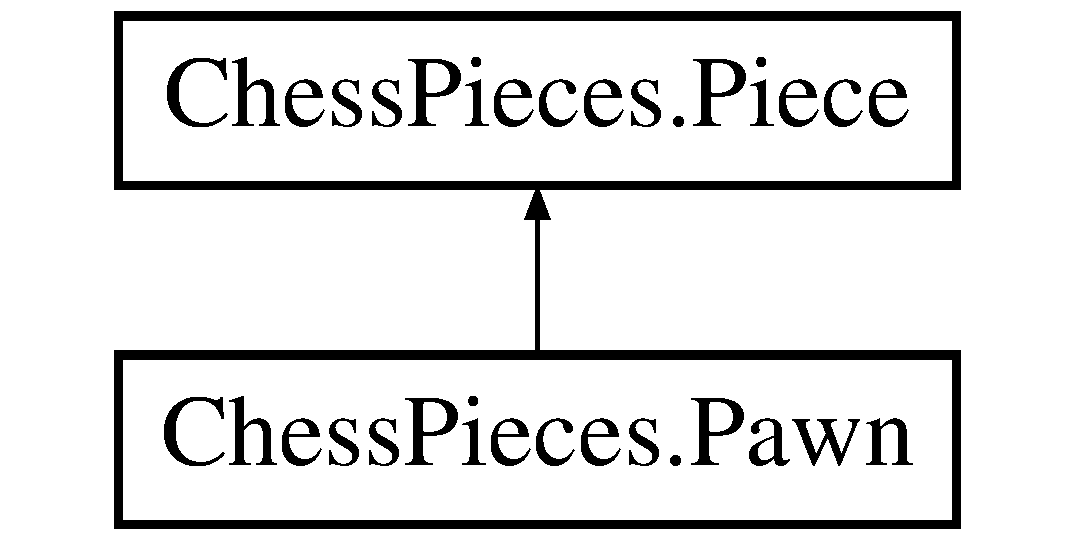
\includegraphics[height=2.000000cm]{class_chess_pieces_1_1_pawn}
\end{center}
\end{figure}
\subsection*{Public Member Functions}
\begin{DoxyCompactItemize}
\item 
{\bfseries Pawn} (\hyperlink{enum_chess_pieces_1_1_color}{Color} col, \hyperlink{class_chess_pieces_1_1_location}{Location} loc)\hypertarget{class_chess_pieces_1_1_pawn_a41a1661e7bb1ef858a8910002441cbdc}{}\label{class_chess_pieces_1_1_pawn_a41a1661e7bb1ef858a8910002441cbdc}

\item 
boolean {\bfseries can\+Move\+To} (\hyperlink{class_chess_pieces_1_1_location}{Location} dest)\hypertarget{class_chess_pieces_1_1_pawn_a33355d440166cb93ec9a2d7f3d093a0b}{}\label{class_chess_pieces_1_1_pawn_a33355d440166cb93ec9a2d7f3d093a0b}

\item 
boolean {\bfseries can\+Move\+To\+Capture} (\hyperlink{class_chess_pieces_1_1_location}{Location} dest)\hypertarget{class_chess_pieces_1_1_pawn_a18f401bcfc49e6617612b9db24ab0848}{}\label{class_chess_pieces_1_1_pawn_a18f401bcfc49e6617612b9db24ab0848}

\item 
void {\bfseries set\+First\+Move} ()\hypertarget{class_chess_pieces_1_1_pawn_a2bcb5a1bbe6489d931faecec6857b786}{}\label{class_chess_pieces_1_1_pawn_a2bcb5a1bbe6489d931faecec6857b786}

\end{DoxyCompactItemize}
\subsection*{Public Attributes}
\begin{DoxyCompactItemize}
\item 
boolean {\bfseries first\+Move}\hypertarget{class_chess_pieces_1_1_pawn_a0d9eb25603976225bc14de9b508c8e62}{}\label{class_chess_pieces_1_1_pawn_a0d9eb25603976225bc14de9b508c8e62}

\end{DoxyCompactItemize}
\subsection*{Additional Inherited Members}


\subsection{Detailed Description}
Created by admin on 1/29/16. 

The documentation for this class was generated from the following file\+:\begin{DoxyCompactItemize}
\item 
src/\+Chess\+Pieces/Pawn.\+java\end{DoxyCompactItemize}

\hypertarget{class_test_1_1_pawn_test}{}\section{Test.\+Pawn\+Test Class Reference}
\label{class_test_1_1_pawn_test}\index{Test.\+Pawn\+Test@{Test.\+Pawn\+Test}}
\subsection*{Public Member Functions}
\begin{DoxyCompactItemize}
\item 
void {\bfseries test\+Can\+Move} ()  throws Exception \hypertarget{class_test_1_1_pawn_test_a0fe8fdca39f3e899cfb2c2db37d499f8}{}\label{class_test_1_1_pawn_test_a0fe8fdca39f3e899cfb2c2db37d499f8}

\end{DoxyCompactItemize}


\subsection{Detailed Description}
Created by admin on 2/2/16. 

The documentation for this class was generated from the following file\+:\begin{DoxyCompactItemize}
\item 
src/\+Test/Pawn\+Test.\+java\end{DoxyCompactItemize}

\hypertarget{class_chess_pieces_1_1_queen}{}\section{Chess\+Pieces.\+Queen Class Reference}
\label{class_chess_pieces_1_1_queen}\index{Chess\+Pieces.\+Queen@{Chess\+Pieces.\+Queen}}
Inheritance diagram for Chess\+Pieces.\+Queen\+:\begin{figure}[H]
\begin{center}
\leavevmode
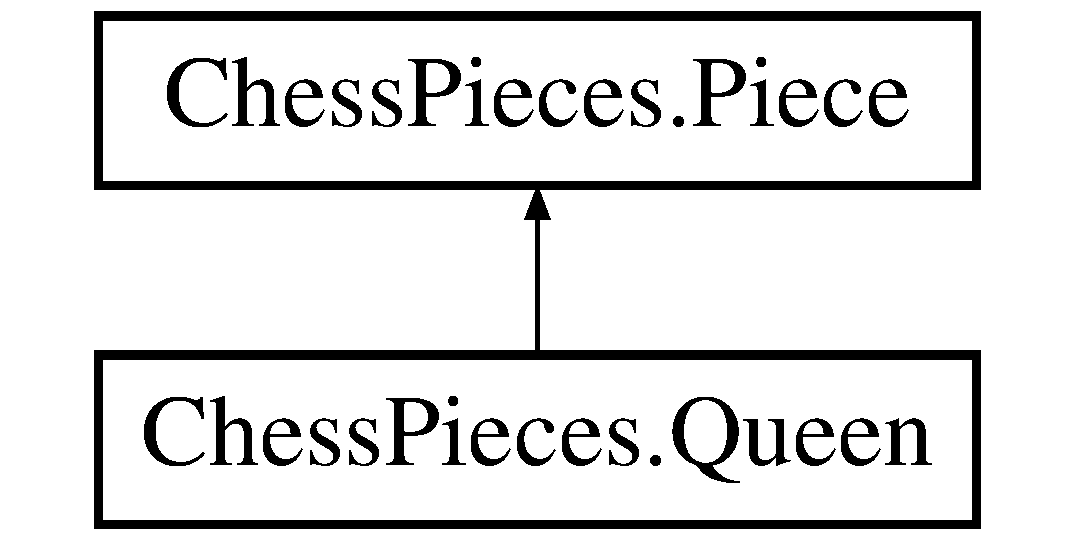
\includegraphics[height=2.000000cm]{class_chess_pieces_1_1_queen}
\end{center}
\end{figure}
\subsection*{Public Member Functions}
\begin{DoxyCompactItemize}
\item 
{\bfseries Queen} (\hyperlink{enum_chess_pieces_1_1_color}{Color} col, \hyperlink{class_chess_pieces_1_1_location}{Location} loc)\hypertarget{class_chess_pieces_1_1_queen_a550dcb93755a0825d6f8b716de4aa07a}{}\label{class_chess_pieces_1_1_queen_a550dcb93755a0825d6f8b716de4aa07a}

\item 
boolean {\bfseries can\+Move\+To} (\hyperlink{class_chess_pieces_1_1_location}{Location} dest)\hypertarget{class_chess_pieces_1_1_queen_a6b8f855055f75a8dcfeec17eb0b7f121}{}\label{class_chess_pieces_1_1_queen_a6b8f855055f75a8dcfeec17eb0b7f121}

\end{DoxyCompactItemize}
\subsection*{Additional Inherited Members}


\subsection{Detailed Description}
Created by admin on 1/29/16. 

The documentation for this class was generated from the following file\+:\begin{DoxyCompactItemize}
\item 
src/\+Chess\+Pieces/Queen.\+java\end{DoxyCompactItemize}

\hypertarget{class_test_1_1_queen_test}{}\section{Test.\+Queen\+Test Class Reference}
\label{class_test_1_1_queen_test}\index{Test.\+Queen\+Test@{Test.\+Queen\+Test}}
\subsection*{Public Member Functions}
\begin{DoxyCompactItemize}
\item 
void {\bfseries test\+Can\+Move\+To} ()  throws Exception \hypertarget{class_test_1_1_queen_test_a6e8fd9cacc0e6d98aa5494489129be08}{}\label{class_test_1_1_queen_test_a6e8fd9cacc0e6d98aa5494489129be08}

\end{DoxyCompactItemize}


\subsection{Detailed Description}
Created by admin on 2/3/16. 

The documentation for this class was generated from the following file\+:\begin{DoxyCompactItemize}
\item 
src/\+Test/Queen\+Test.\+java\end{DoxyCompactItemize}

\hypertarget{class_chess_pieces_1_1_rook}{}\section{Chess\+Pieces.\+Rook Class Reference}
\label{class_chess_pieces_1_1_rook}\index{Chess\+Pieces.\+Rook@{Chess\+Pieces.\+Rook}}
Inheritance diagram for Chess\+Pieces.\+Rook\+:\begin{figure}[H]
\begin{center}
\leavevmode
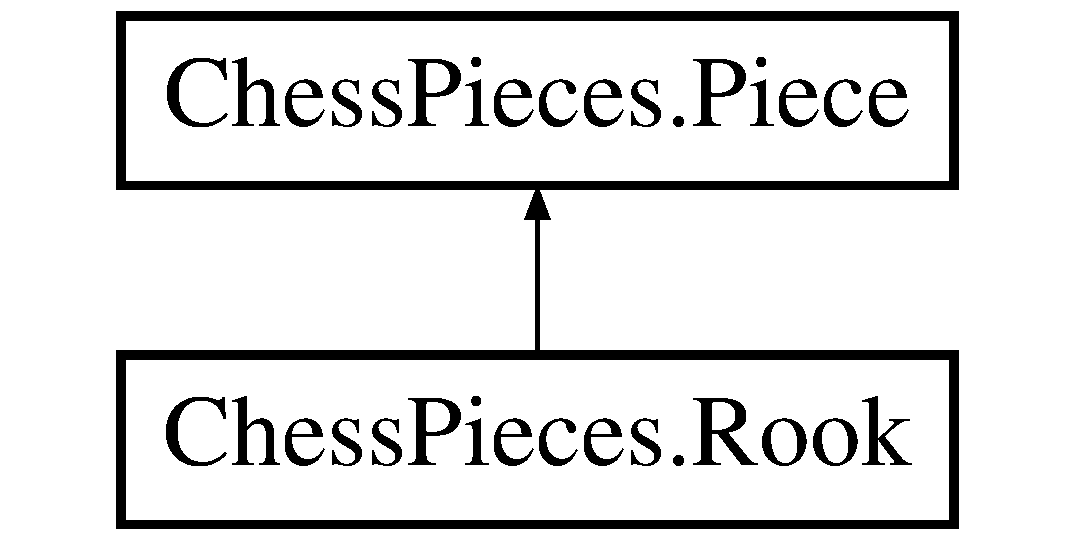
\includegraphics[height=2.000000cm]{class_chess_pieces_1_1_rook}
\end{center}
\end{figure}
\subsection*{Public Member Functions}
\begin{DoxyCompactItemize}
\item 
{\bfseries Rook} (\hyperlink{enum_chess_pieces_1_1_color}{Color} col, \hyperlink{class_chess_pieces_1_1_location}{Location} loc)\hypertarget{class_chess_pieces_1_1_rook_aac17330a776f2de42321192cc08d7ddc}{}\label{class_chess_pieces_1_1_rook_aac17330a776f2de42321192cc08d7ddc}

\item 
boolean {\bfseries can\+Move\+To} (\hyperlink{class_chess_pieces_1_1_location}{Location} dest)\hypertarget{class_chess_pieces_1_1_rook_aa3fc9a4898e072adb1032232a0cdf86d}{}\label{class_chess_pieces_1_1_rook_aa3fc9a4898e072adb1032232a0cdf86d}

\end{DoxyCompactItemize}
\subsection*{Additional Inherited Members}


\subsection{Detailed Description}
Created by admin on 1/29/16. 

The documentation for this class was generated from the following file\+:\begin{DoxyCompactItemize}
\item 
src/\+Chess\+Pieces/Rook.\+java\end{DoxyCompactItemize}

\hypertarget{class_test_1_1_rook_test}{}\section{Test.\+Rook\+Test Class Reference}
\label{class_test_1_1_rook_test}\index{Test.\+Rook\+Test@{Test.\+Rook\+Test}}
\subsection*{Public Member Functions}
\begin{DoxyCompactItemize}
\item 
void {\bfseries test\+Can\+Move\+To} ()  throws Exception \hypertarget{class_test_1_1_rook_test_ab70917a02c7a65f894595975a96678db}{}\label{class_test_1_1_rook_test_ab70917a02c7a65f894595975a96678db}

\end{DoxyCompactItemize}


\subsection{Detailed Description}
Created by admin on 2/3/16. 

The documentation for this class was generated from the following file\+:\begin{DoxyCompactItemize}
\item 
src/\+Test/Rook\+Test.\+java\end{DoxyCompactItemize}

\hypertarget{class_board_and_game_1_1_square}{}\section{Board\+And\+Game.\+Square Class Reference}
\label{class_board_and_game_1_1_square}\index{Board\+And\+Game.\+Square@{Board\+And\+Game.\+Square}}
\subsection*{Public Member Functions}
\begin{DoxyCompactItemize}
\item 
{\bfseries Square} (\hyperlink{class_chess_pieces_1_1_location}{Location} loc, \hyperlink{enum_chess_pieces_1_1_color}{Color} col)\hypertarget{class_board_and_game_1_1_square_a92a2aefbb8e9f1fc3d84bb84e3500c4a}{}\label{class_board_and_game_1_1_square_a92a2aefbb8e9f1fc3d84bb84e3500c4a}

\item 
void {\bfseries delete\+Piece} ()\hypertarget{class_board_and_game_1_1_square_a8c9a929e2f8f4f6f663ab37a15d61cd0}{}\label{class_board_and_game_1_1_square_a8c9a929e2f8f4f6f663ab37a15d61cd0}

\item 
void {\bfseries set\+Piece} (\hyperlink{class_chess_pieces_1_1_chess_piece}{Chess\+Piece} new\+Piece)\hypertarget{class_board_and_game_1_1_square_a7855ecbf83baff922e770feb6fcc5179}{}\label{class_board_and_game_1_1_square_a7855ecbf83baff922e770feb6fcc5179}

\item 
void {\bfseries set\+Color} (\hyperlink{enum_chess_pieces_1_1_color}{Color} col)\hypertarget{class_board_and_game_1_1_square_ae75a4148f6b31d3cf75693b142fab8e5}{}\label{class_board_and_game_1_1_square_ae75a4148f6b31d3cf75693b142fab8e5}

\item 
\hyperlink{enum_chess_pieces_1_1_color}{Color} {\bfseries get\+Color} ()\hypertarget{class_board_and_game_1_1_square_a2c18545b412082261de04e24afe927b1}{}\label{class_board_and_game_1_1_square_a2c18545b412082261de04e24afe927b1}

\item 
\hyperlink{class_chess_pieces_1_1_chess_piece}{Chess\+Piece} {\bfseries get\+Piece} ()\hypertarget{class_board_and_game_1_1_square_ac5a6c5410d50faba7650fa5f9db123c9}{}\label{class_board_and_game_1_1_square_ac5a6c5410d50faba7650fa5f9db123c9}

\item 
boolean {\bfseries has\+Piece} ()\hypertarget{class_board_and_game_1_1_square_a9491979b8d640082f8bcdcd5d1f1b270}{}\label{class_board_and_game_1_1_square_a9491979b8d640082f8bcdcd5d1f1b270}

\end{DoxyCompactItemize}


\subsection{Detailed Description}
Created by admin on 1/29/16. 

The documentation for this class was generated from the following file\+:\begin{DoxyCompactItemize}
\item 
src/\+Board\+And\+Game/Square.\+java\end{DoxyCompactItemize}

%--- End generated contents ---

% Index
\backmatter
\newpage
\phantomsection
\clearemptydoublepage
\addcontentsline{toc}{chapter}{Index}
\printindex

\end{document}
